\newpage
\section{Autenticazione}

\label{Autenticazione}
\begin{figure}[ht]
	\centering
	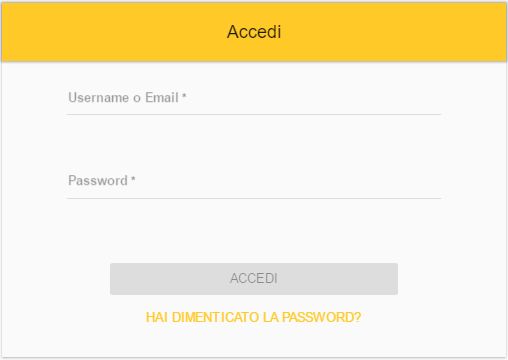
\includegraphics[scale=0.65]{img/autenticazione.png}
	\caption{Autenticazione}
\end{figure}
\FloatBarrier

Effettuata la registrazione è possibile autenticarsi al sistema. Compilati correttamente i campi \textit{Username o E-mail} e \textit{Password}, il bottone \textit{Accedi} viene abilitato dando la possibilità di autenticarsi. Se l'autenticazione va a buon fine, all'utente viene presentata l'Home Page con alcune nuove voci all'interno della barra del menù a destra. Se l'utente appena autenticato è di tipo \textit{normale} saranno presenti le seguenti voci, le quali rappresentano le operazioni che l'utente è abilitato ad eseguire:
\begin{itemize}
	\item Gestione profilo;
	\item Gestione domande;
	\item Cambia lingua.
\end{itemize}
Se invece l'utente è di tipo \textit{pro}, gli verranno presentate le seguenti voci:
\begin{itemize}
	\item Gestione profilo;
	\item Gestione questionari;
	\item Gestione domande;
	\item Cambia lingua. 
\end{itemize}